% Author: Surya Mohan Kamini
% Roll No.: 140010049
% Email: suryamohan@iitb.ac.in
% Date: 22-10-2016

\documentclass[12pt, a4paper]{article}

\usepackage{amsmath}
\usepackage{graphicx}

\usepackage{url}
\usepackage[bookmarks=true]{hyperref}
\usepackage{bookmark}


\begin{document}

\title{Mass Spring Damper System}
\author{Surya Mohan Kamini\\
	Roll No. 140010049\\
	\texttt{suryamohan@iitb.ac.in}
	}
\date{\today}
\maketitle

{\tableofcontents}
{\listoffigures}

\pagebreak

\begin{abstract}
This is a report of simulation of Mass Spring Damper System. An example system is taken, a plot of displacement vs time and  velocity vs time is given.
There is also an animation of Mass Spring system.The coding part was done in python.
\end{abstract}

\section{Source Code}
\subsection{Repository}
The source code for Mass Spring Damper System  can be found at following repository:\\
\url{https://github.com/theyoungsurya/mass_spring_damper_system.git}

\subsection{Dependencies}
The souce code at above mentioned repo is based on:
\begin{itemize}
\item Python 2
\item pdfTeX 3.14159265-2.6-1.40.16
\item matplotlib 1.5.3
\item numpy 1.11.2
\item GNU Make 4.1
\end{itemize}



\section{Introduction}
    Mass Spring Damper System is one of the simplest vibratory system. It consists of a mass $m$ attached to an immovable support by means of a spring of stiffness $k$. The mass is constrained to translational motion in X-axis so that its change of position from an intial reference is completely described by the value of a single quantity $x$. This is why this type of systems are called $single$ $degree$ $of$ $freedom$ $systems$.\\ 

If the mass is displaced from its equilibrium position and allowed to oscillate free from further external forces. The system is said to be in free vibration. It also can be in forced vibration i.e, a continuing action of force on system or the foundation of the system may be in continuous motion. Free and Forced vibrations are discussed below.
\subsection{Free vibrations without damping}
\begin{figure}[h]
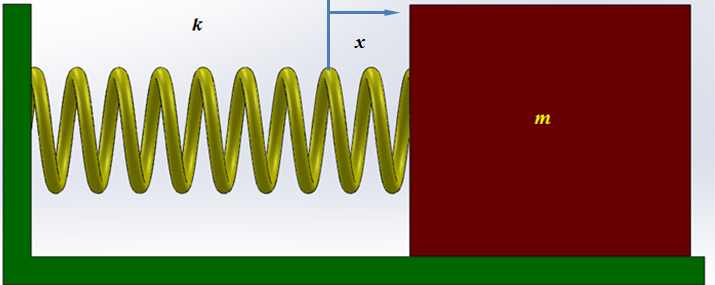
\includegraphics[width=0.8\textwidth]{Undamped_free_vibrations.png}
\caption{Undamped Free Vibration of Spring Mass system (Roll No. 140010049)}
\label{fig:undamped}
\end{figure}
Consider first the free vibration of undamped system shown in the  figure \ref{fig:undamped}. By Newton's law as it is in equilibrium the forced exerted by mass due to inertia is equal to the force exerted by spring. And the frequency at which it oscillation when disturbed is called $natural$ $frequency$\\
\begin{equation} 
m\ddot{x} + kx = 0
\label{undamped-newton}
\end{equation}

\subsection{Free Vibration with viscous damping}
\begin{figure}[h]
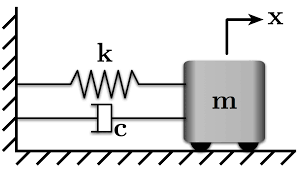
\includegraphics[width=0.7\textwidth]{Damped_free.png}
\caption{Free Vibration of Spring Mass system with visous damping (Roll No. 140010049)}
\label{fig:damped}
\end{figure}
Figure \ref{fig:damped} shows a mass spring system with a viscous damper. The differential equation for this system written as the following:\\
\begin{equation} 
m\ddot{x} + c\dot{x} + kx = 0
\label{damped-newton}
\end{equation}
Because the viscous damping is directly proportional to the velocity of the body. $c$ is called $Damping$ $Coefficient$. Depending on the value of $c/\sqrt{km}$ damping is of three types critical damping , over-damping , under-damping.\\

\subsection{Forced Vibration with viscous damping}
\begin{figure}[h]
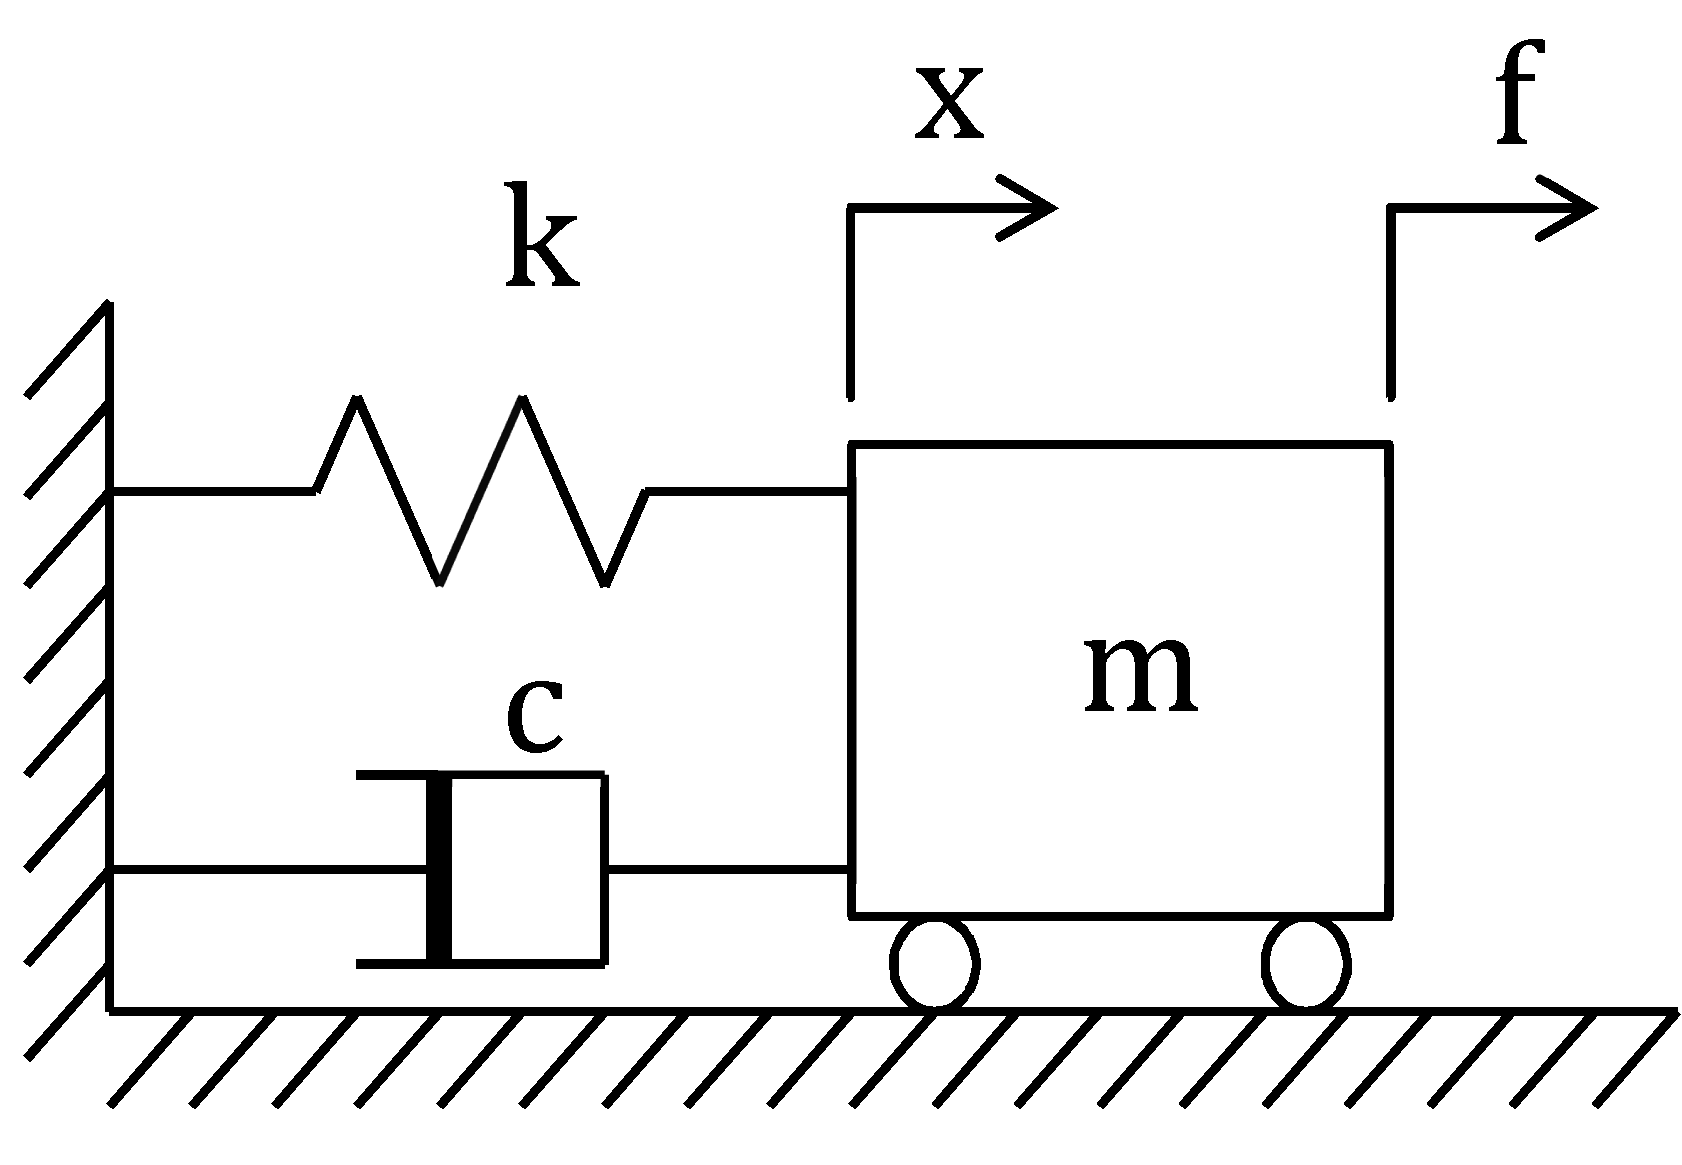
\includegraphics[width=0.7\textwidth]{Forced_damped.png}
\caption{Forced Vibration of Spring Mass system with visous damping (Roll No. 140010049)}
\label{fig:forced_damped}
\end{figure}
Similary, the equation of motion of the spring mass system with viscous damping when an excitation force $F$ is applied as shown in figure
\ref{fig:forced_damped} is written by applying the newton's law and is written as the following differential equation:\\
\begin{equation} \label{sec-ord-eq}
m\ddot{x}+c\dot{x}+kx=F
\end{equation}
where $x$ is position of at time  $t$. $c$ and $k$ are damping coefficient of system and stiffness constant of spring respectively.\\



\section{Example:}
\begin{figure}[h]
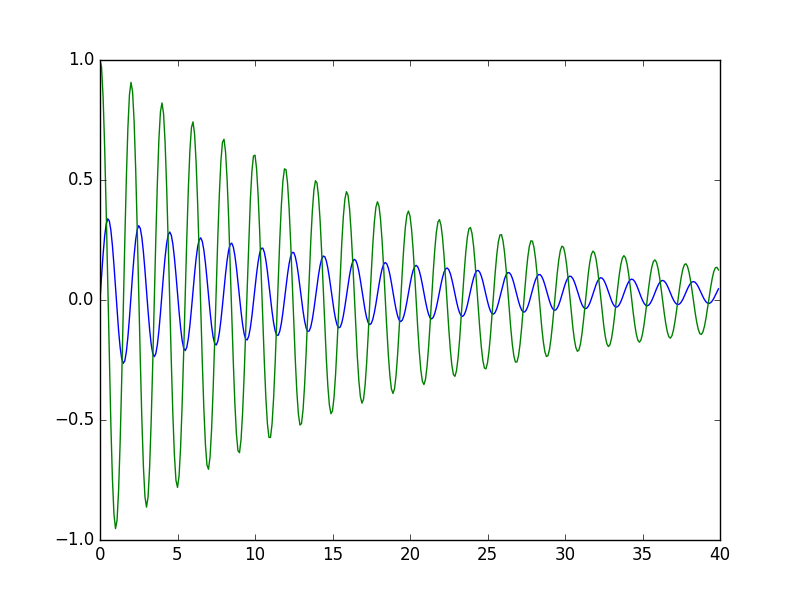
\includegraphics[width=0.8\textwidth]{../output/Disp&Vel_vs_time.png}
\caption{Displacement, Velocity vs Time (Roll No. 140010049)}
\label{fig:exampleplot}
\end{figure}

The figure \ref{fig:exampleplot} shows the solution plot of Mass Spring Damper System. The plot depicts $x$ vs. $t$ and $v$ vs. $t$ respectively. Typically $F$ is a harmonic but we have considered a system with constant force acting on it.Solving the second order differential equation for analytical solution is very difficult. So it  was solved numerically using RK4 (Range-Kutta) method.\\*

The parameters used for this example are:\\*
$m$ = 100.0, $k$ = 1000.0, $c$ = 10.0, $t$ = 40.0, $dt$ = 0.1, $x-initial$ = 1.5, $v-intial$ = 3.0, $F$ = 30.0\\*
All quantities in SI units.


\href{run:Animation.html}{Click to View Animation}
The link may not work in firefox due to lack of plugin support. If so open animation video in this directory directly.(The link works in Chrome and Chromium). 

\end{document}
